\documentclass[letterpaper,10pt]{article}
\usepackage{graphicx}
\usepackage{osameet2}
\usepackage{amsmath,amssymb}

\begin{document}
\title{Automated Design of Nanophotonic Waveguide-to-Waveguide Couplers}
\author{Jesse Lu and Jelena Vu\v{c}kovi\'{c}}
\address{Stanford University, Stanford, California, USA.}
\email{jesselu@stanford.edu}

\maketitle
\begin{abstract}
We demonstrate a design algorithm which automatically generates 
wavelength-scale coupling devices between arbitrary waveguide modes with high
efficiency.
Our algorithm is fast ($\sim$20 min.), can be extended to multiple dimensions,
 and requires no trial-and-error.
\end{abstract}
\ocis{230.7370, 130.3990.}

% Importance of problem.
\section{Motivation}
In order to route and process optical information on-chip, it is absolutely
critical to be able to efficiently transfer photons from one waveguide mode
to another.
% NEED TO CITE HERE!
However, current strategies either 
1) require large device areas and tunable material parameters,
2) are only applicable to effectively 1D systems, or 
3) operate on brute force parameter search.

% Capabilities of our algorithm.
We present an algorithm that quickly ($\sim$20 min.) designs high efficiency
($\sim$95\% conversion) nanophotonic waveguide couplers in two dimensions.
The resulting devices are extremely compact, on the order of only 1-2 vacuum 
wavelengths per side, and can couple between seemingly arbitrary waveguide 
modes.
Notably, neither trial-and-error nor the modeling of device subcomponents 
is needed.

% How it works.
\section{Method}
The algorithm operates by calculating the boundary electromagnetic fields
needed for perfect operation (100\% coupling efficiency), and then varying the 
interior fields and permittivities to reproduce those boundary fields.  
Numerically, we fix $H({border}) = H_\text{perfect}$,
and then minimize the residual in the electromagnetic wave equation,
$\| \nabla \times \epsilon^{-1} \nabla \times H - \mu \omega^2 H \|^2$, 
by varying both $H({interior})$ (interior magnetic field) and 
$\epsilon$ (permittivity).

Note that the algorithm actually places much greater emphasis on achieving 
perfect device performance than even satisfying physics (the wave equation)!
Specifically, it is this ``objective-first'' approach, 
coupled with the boundary field formulation, 
that greatly speeds up the design process by eliminating the need to  
repeatedly solve the wave equation.

Lastly, we validate our designs in simulation 
(finite-difference frequency-domain, 2D tranverse electric mode) 
by exciting the input waveguide mode and then calculating the transmitted power
in the desired output waveguide mode.

\section{Results}
Figs. 1, 2 and 3 show the result of our algorithm, as applied to the design 
of nanophotonic waveguide couplers in two dimensions.  
All devices are extremely compact, and yet exhibit high coupling efficiency; 
even in spite of significant differences in mode size and mode symmetry.

Lastly, for numerical reasons, we allow values of $\epsilon$ to vary 
continuously between $\epsilon_\text{air} = 1$ and 
$\epsilon_\text{silicon} = 12.25$, even though discrete values are more
amenable to fabrication. 
Forcing discreteness in $\epsilon$ will be investigated in future work.


This work has been supported in part by the 
AFOSR MURI for Complex and Robust On-chip Nanophotonics (Dr. Gernot Pomrenke),
grant number FA9550-09-1-0704.
% \begin{thebibliography}{99}
% \bibitem{lipson} Almeida et al, Optics Letters \textbf{28}, 1302-1304 (2003).
% \end{thebibliography}


% Coupling efficiency
% Design time
% Size of the device
% Frequency
\begin{figure}[htbp]
    \centering
    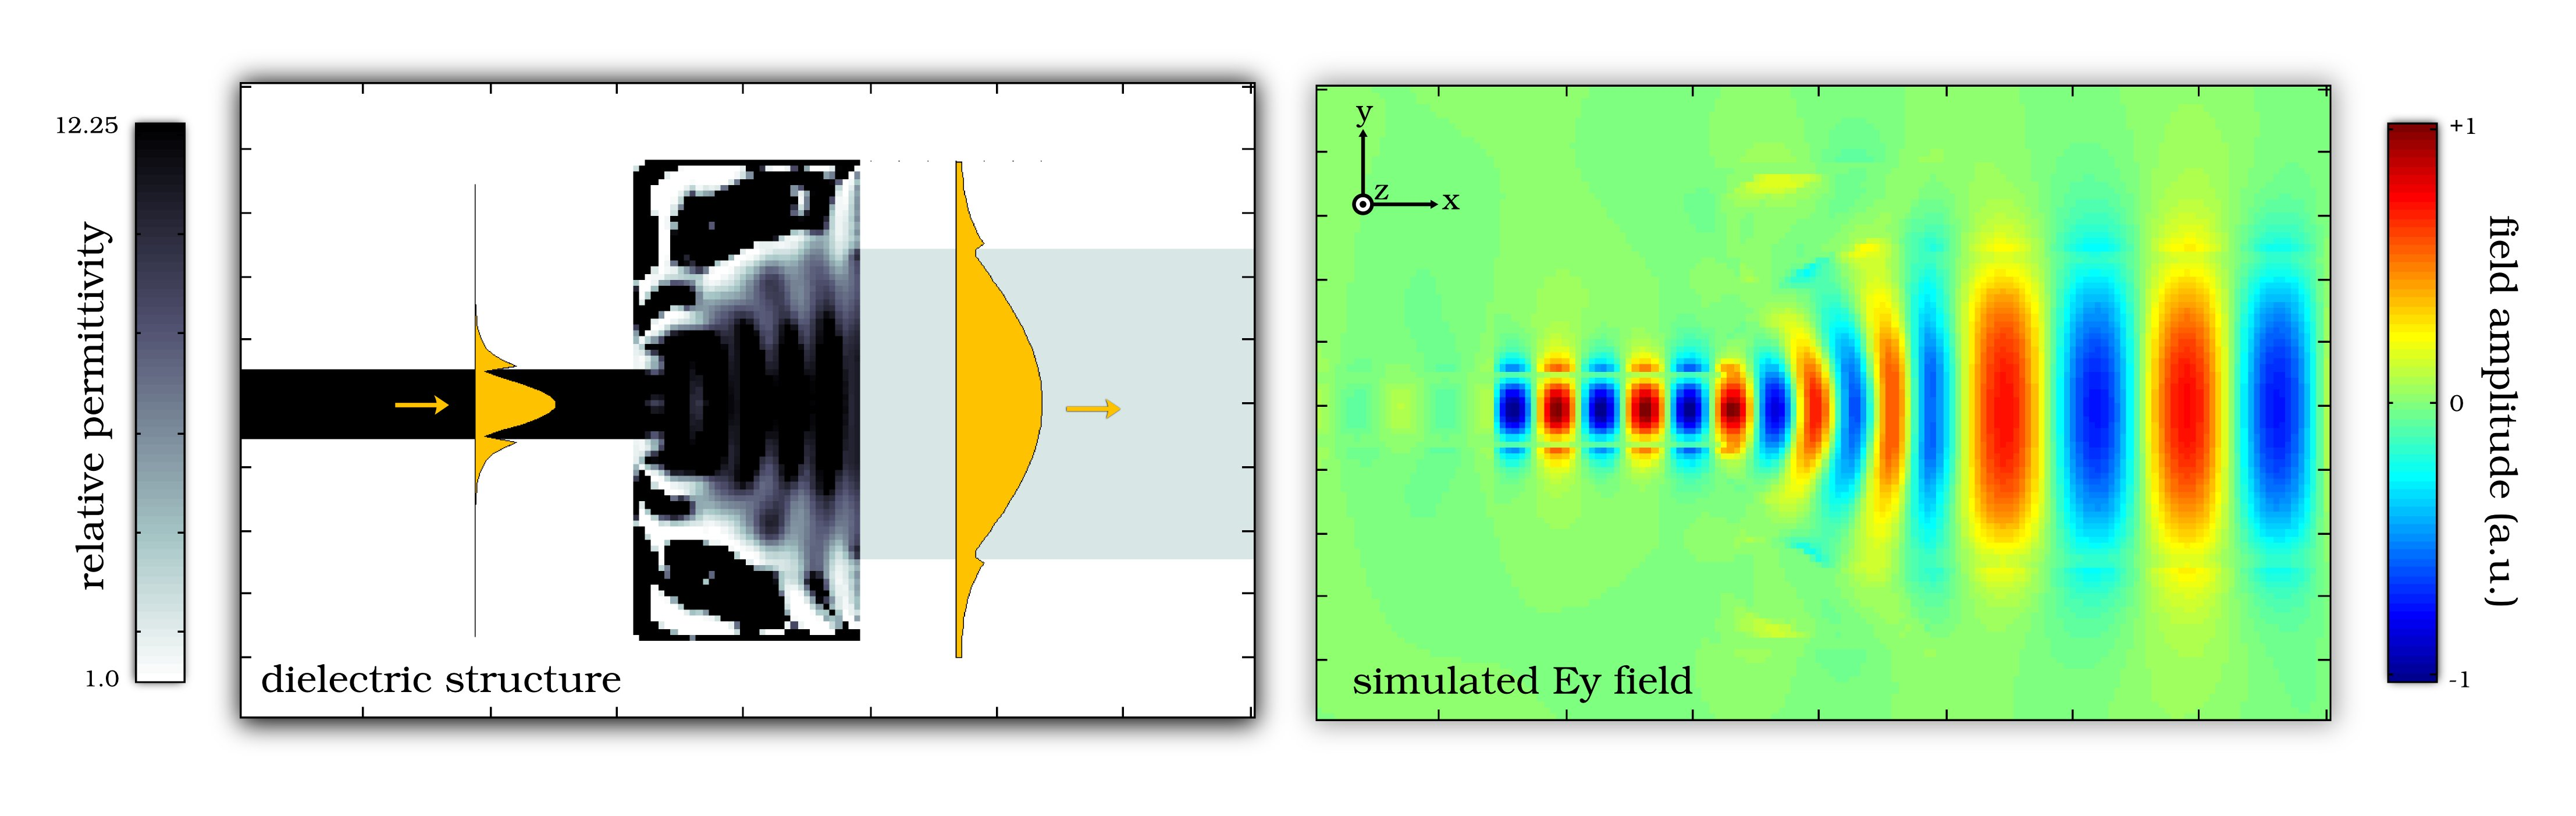
\includegraphics[width=0.9\textwidth]{fig/fiber.jpg}
    \caption{Waveguide coupler for a wide, low-index waveguide. 
        The dielectric structure of the coupler and surrounding input and
        output waveguides is shown on the left, while the simulation
        validating our results is shown on the right.
        The coupler converts $96.3\%$ of the input power to the
        designated output mode.
        The device is extremely compact, 
        convering only $36 \times 66$ grid points,
        where the vacuum wavelength is 42 grid points.
        Computation time was 20 minutes on a personal computer.}
\end{figure}
\begin{figure}[htbp]
    \centering
    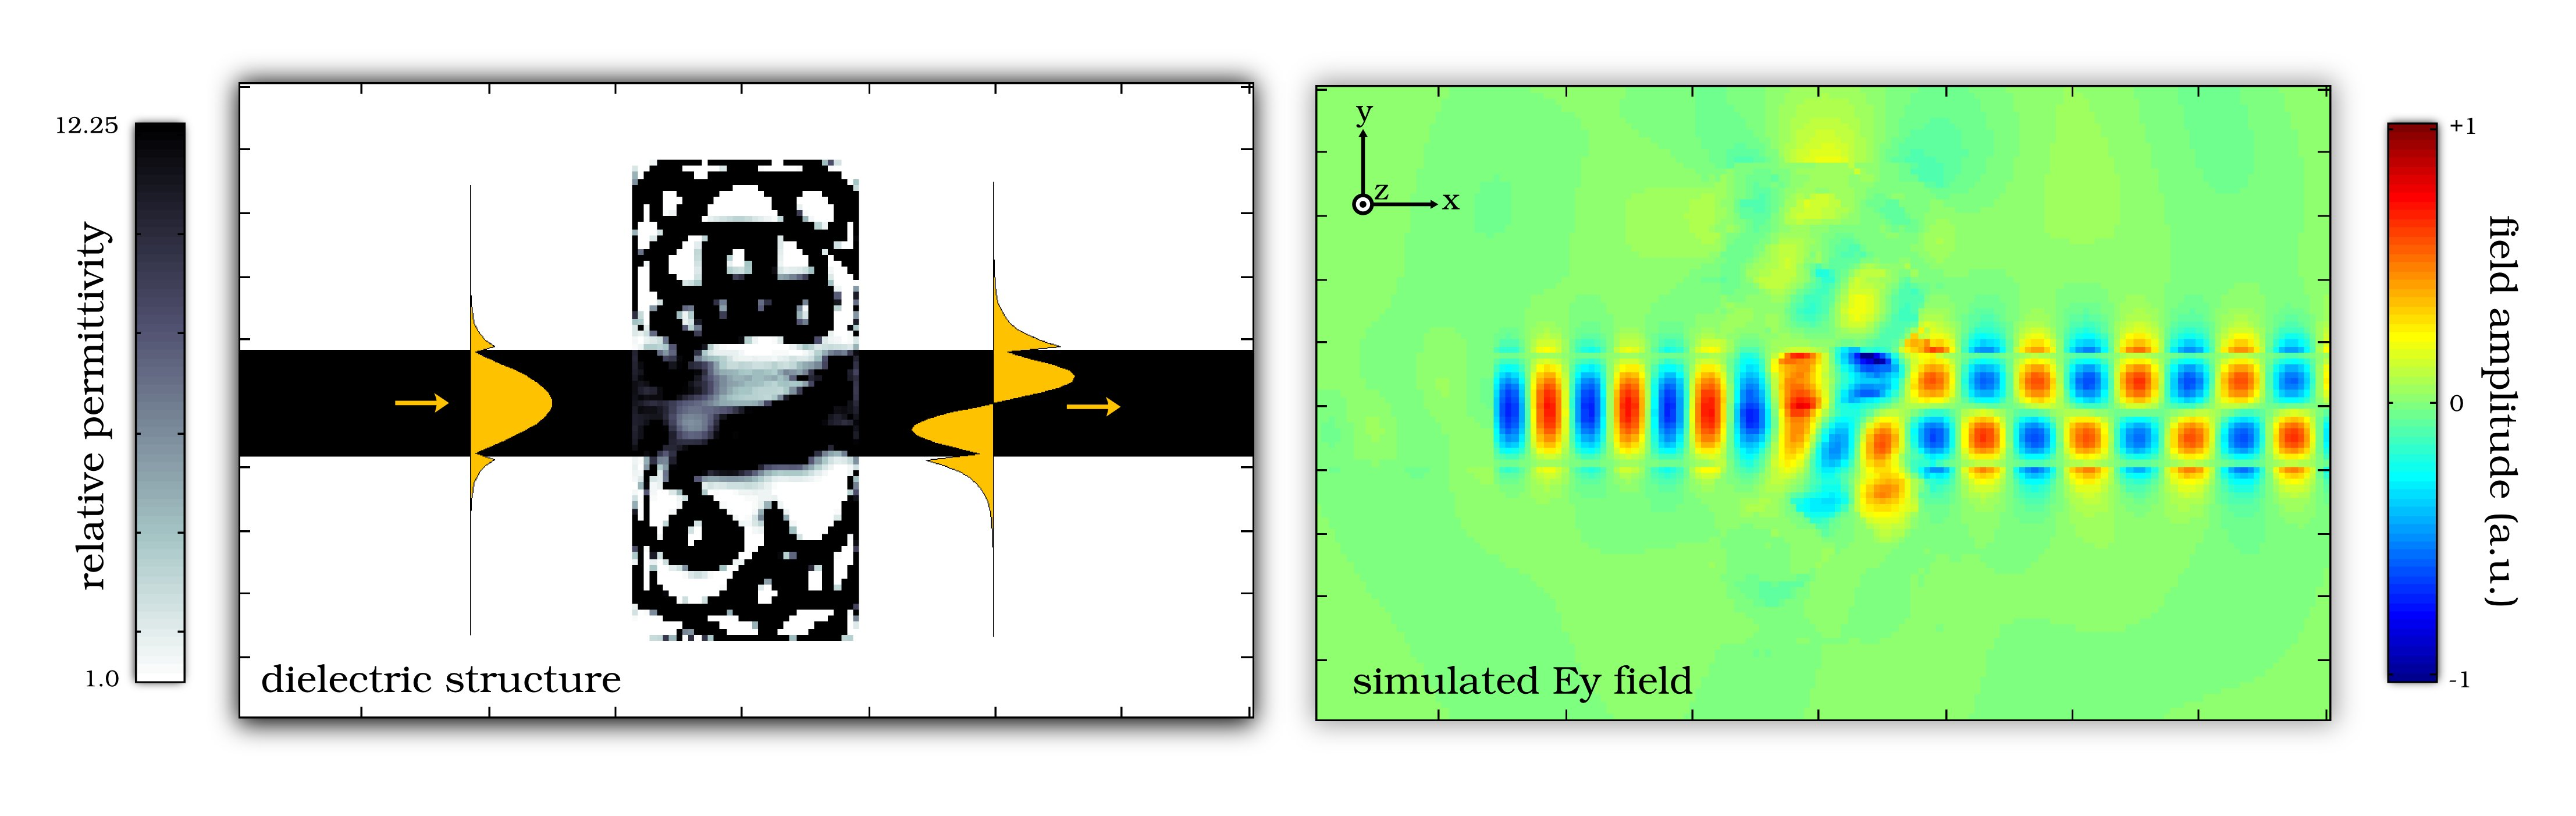
\includegraphics[width=0.9\textwidth]{fig/mode-conv.jpg}
    \caption{Coupler that converts the fundamental waveguide mode to the
        second-order waveguide mode.
        This problem is quite difficult since the two modes are of 
        opposite symmetry.
        For example, adiabatic approaches cannot be applied to this case.
        However, our method produces a device 
        (which has the same dimensions and vacuum wavelength as Fig. 1) 
        which achieves a coupling efficiency of $95.5\%$. 
        Computation time was extended to 50 minutes to improve efficiency.
        }
\end{figure}
\begin{figure}[htbp]
    \centering
    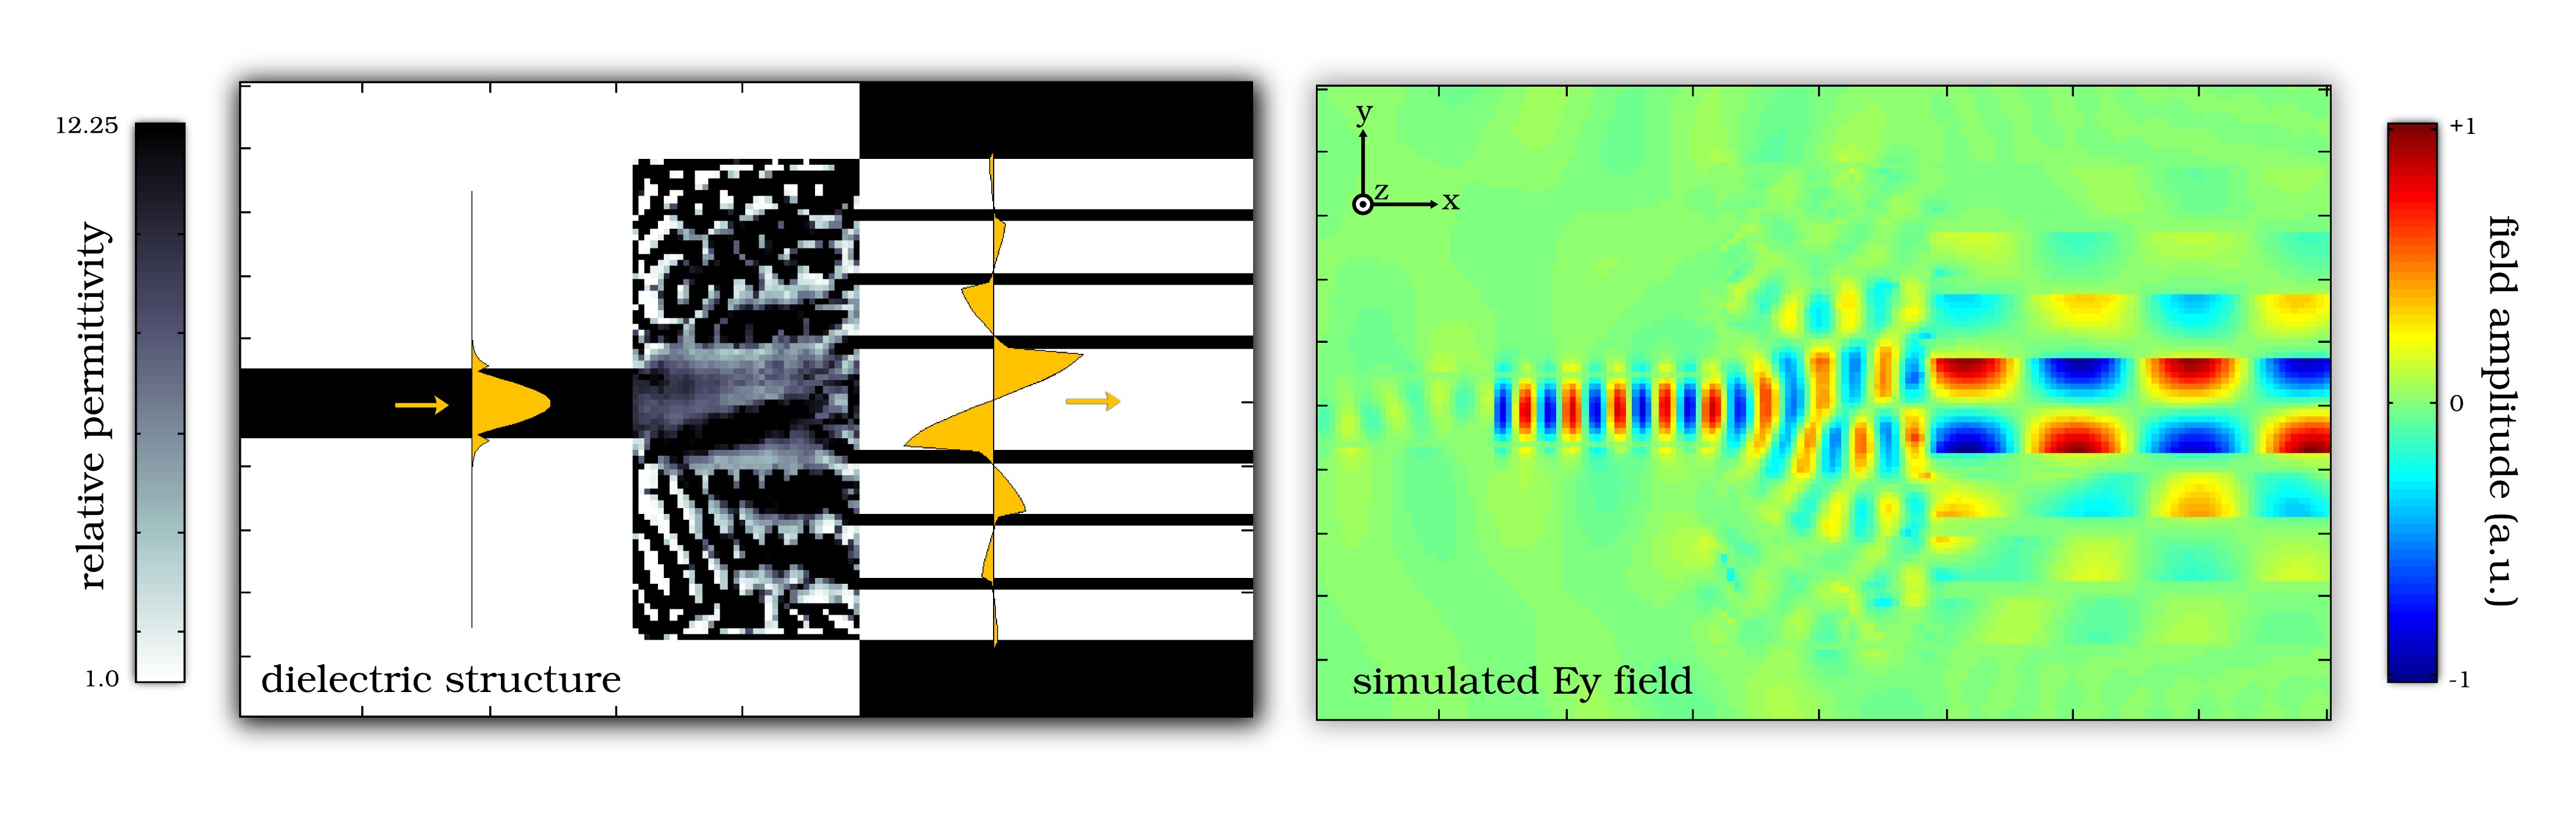
\includegraphics[width=0.9\textwidth]{fig/air-core.jpg}
    \caption{Coupler to an air-core mode.
        Here, not only are the modes of opposite symmetry,
        but the output waveguide operates on a fundamentally different
        principle (guided by Bragg reflection) than the input waveguide 
        (index guided).
        The device still achieves an efficiency of $83.3\%$, demonstrating the
        versatility of our method.
        The vacuum wavelength is 25 grid points, 
        while the device footprint is still $36 \times 66$ grid points.
        Computation time was 20 minutes.
        }
\end{figure}
\end{document}

